\subsection{Bestimmung des Massendurchsatzes}

Zur Bestimmung des Massendurchsatzes muss zuvor die Verdampfungswärme L des Gases bestimmt werden. Dies geschieht, in dem zuvor vom Manometer aufgenommene
Druck-Temperetur Wertepaare gegeneinander aufgetragen werden und hierüber eine lineare Ausgleichsrechnung erfolgt. Die Wertepaare hierzu finden sich in \autoref {tab:temppa}.
Die Verdampfungswärme L lässt sich dann durch die Steigung $a$ der linearen Ausgleichsgeraden und der Gaskonstanten $R$ durch $L = a \cdot R$, wobei die Ausgleichsgerade durch
\begin{equation}
  \label{eqt:Ausgleichsgerade}
  y = a \cdot x + b,
\end{equation}
wobei y hier der Druck und x die Temperatur, womit a die Zunahme des Druckes bei steigender Temperatur und b den Druck bei $ T = 0$.
Die Parameter ergeben sich durch
\begin{equation}
\label{eqt:b}
  b = \frac {\sum_{i=1}^n (x_i - \overline{x}) \cdot (y_i - \overline{y})}{\sum_{i=1}^n (x_i - \overline{x})^2}
\end{equation}
und 
\begin{equation}
\label{eqt:a}
  a = \overline{y} - b \cdot \overline{x}, 
\end{equation}
wobei $x_i$ die Temperaturwerte und $y_i$ die Druckwerte (beides zu sehen in \autoref{tab:temppa}) sind. Die dazugehörigen Mittelwerte $\overline{x}$ und $\overline{y}$, zu n Werten (hier: $n = 10$), berechnen sich über
\begin{equation}
\label{eqt:mittelwert}
  \overline{x} = \frac {1}{n} \sum_{i=1}^n x_i . 
\end{equation}
Somit ergeben sich nach Gleichungen \eqref{eqt:b}, \eqref{eqt:a} und \eqref{eqt:mittelwert}
\begin{equation}
    b = 9.9 \pm 0.1  
\end{equation}
und 
\begin{equation}
 \lvert a \rvert = 2408 \pm 30. 
\end{equation}
Die sich dadurch nach Gleichung \eqref{eqt:Ausgleichsgerade} ergebene Gerade ist in Abbildung \ref{fig:dampf} zu sehen.
Zur Bestimmung von L ist neben der Steigung der Verdampfungkurve, die Gaskonstante $R = 8,314 \frac{\symup{J}}{\symup{mol} \symup{K}}$ nötig.
Mit der Relation
\begin{equation}
  L = \lvert a \rvert R
\end{equation}
lässt sich die Verdampfungswärme zu
\begin{equation}
  L =  (20020.69 \pm 246.62)\frac{\symup{J}}{\symup{mol} \symup{K}}
\end{equation}
berechnen.
Zur weiteren Berechnung muss die Verdampfungswärme durch die molare Masse geteilt werden, um L in einer zur weiteren Berechnung sinnvollen Einheit zu erhalten, wobei 
die molare Masse von Dichlordiflourmethan $M = 120,91 \frac{\symup{g}}{\symup{mol} }$ \cite{chemie} beträgt, womit
\begin{equation}
  L =  (165.58 \pm 2.04) \frac{\symup{J}}{\symup{g} \symup{K}}
\end{equation}
beträgt. 

\begin{table}[!htp]
\centering
\caption{Die Temperatur - Druck Wertepaare.}
\label{tab:temppa}
\begin{tabular}{c c}
\toprule $p$ / bar & $T$ / K \\
\midrule
3.0 & 273.15 \\
3.8 & 279.15 \\
4.0 & 281.15 \\
4.8 & 287.15 \\
5.5 & 293.15 \\
6.0 & 295.15 \\
7.0 & 301.15 \\
7.4 & 303.15 \\
9.5 & 313.15 \\
12.0& 323.15 \\
\bottomrule
\end{tabular}
\end{table}

\begin{figure}
  \centering
  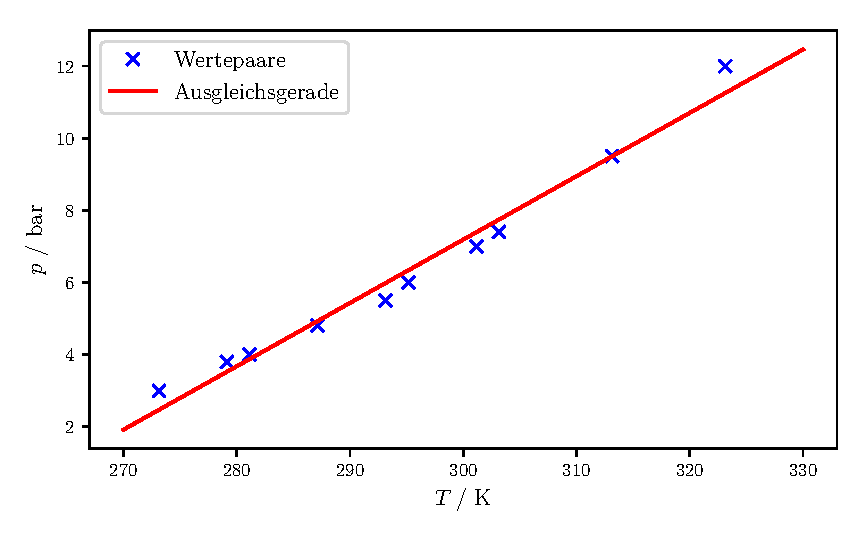
\includegraphics{plot-L.pdf}
  \caption{Verdampfungkurve von Dichlordiflourmethan.}
  \label{fig:dampf}
\end{figure}

Nach \eqref{eqt:massendurchsatz} berechnen sich dann die Massendurchsätze, wie in \autoref{tab:massendurchsatz} zu sehen.
Der Fehler des Massendurchsatzes lässt sich nach Gleichung \eqref{eqt:fehlerfortpflanzung} durch
\begin{equation}
\sigma_{\frac{dm}{dt}} = \sqrt{\Bigl(\frac {C_w + C_k}{L}\Bigr)^2 \sigma_{\frac{dT_2}{dt}}^{2} + \Bigl(\frac{1}{L} \frac{dT_2}{dt}\Bigr )^2 \sigma_{C_w}^{2} + \Bigl(- \frac {C_w + C_k}{L^2}\frac{dT_2}{dt} \Bigr)^2 \sigma_L^{2} }
\end{equation}
berechnen, wobei $\sigma_{\frac{dT_2}{dt}}$ der Fehler der Differentiale $\frac{dT_2}{dt}$, $\sigma_L$ der Fehler von L und $\sigma_{C_w}$ der Fehler der Wärmekapazität des Wassers $C_w$ ist.
\begin{table}[!htp]
  \centering
  \caption{Die Massendurchsätze zu den Temperaturen.}
  \label{tab:massendurchsatz}
  \begin{tabular}{
    S[table-format=2.3] @{${}\pm{}$} S[table-format=1.3]
    S[table-format=2.1] @{${}\pm{}$} S[table-format=1.1]}
    \toprule
    \multicolumn{2}{c}{$T_2 / dt$ / K}  & \multicolumn{2}{c}{$dm/dt$ / g/s } \\
    \midrule
     -0.021 & 0.002 & -1.7 & 0.2 \\
     -0.027 & 0.005 & -2.2 & 0.4 \\
     -0.024 & 0.007 & -1.9 & 0.6 \\
     -0.010 & 0.010 & -0.8 & 0.8 \\
    \bottomrule
  \end{tabular}
\end{table}